\section{Fouriertransformation}


\subsection{Linearkombinationen gleichperiodischer Funktionen}

Linearkombinationen periodischer Funktionen derselben Periode sind ebenfalls
periodisch mit dieser Periode. Oder formal: Seien $f$ und $g$ zwei Funktionen
mit derselben Periode $p$ und $a$ sowie $b$ zwei Konstanten. Dann ist auch die
Funktion
$$af+bg$$
periodisch mit der Periode $p$.


\subsection{Fourier-Entwicklung periodischer Funktionen}


\subsubsection{Sinus-Kosinus-Form}
Wir betrachten ein stückweise stetiges, mit der Grundperiode $T$
periodisches Signal $s$. Dann heisst die Funktion
$$f_n := t \mapsto a_0 + \sum_{k=1}^n \left[ a_k \cos(k\omega_1t)
    + b_k\sin(k\omega_1t)\right]$$
mit
$$\omega_1 = \frac{2\pi}{T}$$
$$a_0 = \frac{1}{T} \int\limits_0^T s(t) dt$$
$$a_k = \frac{2}{T} \int\limits_0^T s(t) \cos(k\omega_1t) dt$$
$$b_k = \frac{2}{T}\int\limits_0^T s(t) \sin(k\omega_1t) dt$$
für $k \in \{1...n\}$ seine \emph{Fourierentwicklung} der Ordnung $n$.

$\omega_1$ heisst die \emph{Grundkreisfrequenz}, $a_0$ die
\emph{Konstante}, $a_k$ und $b_k$ die \emph{Koeffizienten}.

\subsubsection{Spektral-Form}
Neben dieser sogenannten \emph{Sinus-Kosinus-Form} gibt es die für die
Praxis wichtigere \emph{Amplituden-Phasen-Form} oder \emph{Spektral-Form}
$$f_n := t \mapsto A_0 + \sum_{k=1}^n A_k \cos(k\omega_1t - \varphi_k)$$
Die Bestimmungsstücke der Amplituden-Phasen-Form können nicht direkt berechnet
werden, sondern auf dem Umweg über die Koeffizienten der Sinus-Kosinus-Form.
Dabei gilt folgender Zusammenhang:
\begin{itemize}
    \item $A_0 = a_0$
    \item Ein Punkt in der Ebene, der die kartesischen Koordinaten $(a_k, b_k)$
    hat, hat die Polarkoordinaten $(A_k, \varphi_k)$
\end{itemize}


\subsection{Koordinatentransformation Kartesisch / Polar}

Koordinaten aus dem Kartesischen- oder Polarkoordinatensystem können
folgendermassen transformiert werden:

\begin{figure}[H]
    \centering
    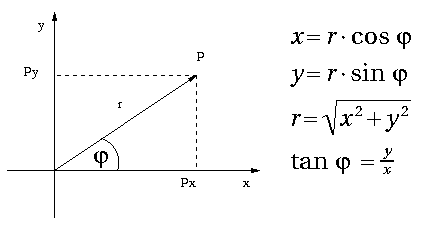
\includegraphics[scale=0.5]{pictures/koordinatentransformation.png}
    \caption{Zusammenhänge Kartesische Koordinaten / Polarkoordinaten}
\end{figure}

Übertragen auf die Fourierreihen entspricht in der Grafik:
\begin{itemize}
    \item $a_k$ = $x$ (Sinus-Kosinus-Form)
    \item $b_k$ = $y$ (Sinus-Kosinus-Form)
    \item $A_k$ = $r$ (Spektralform)
    \item $\phi_k$ = $\phi$ (Spektralform)
\end{itemize}

Um den Winkel $\varphi$ im Interval $(-\pi, \pi]$ zu berechnen, gibt es mehrere
Möglichkeiten. Mithilfe des Arkustangens:
$$\varphi = \begin{cases}
    \arctan\frac{y}{x} & \mathrm{f\ddot ur}\ x > 0\\
    \arctan\frac{y}{x} + \pi & \mathrm{f\ddot ur}\ x < 0,\ y \geq 0\\
    \arctan\frac{y}{x} - \pi & \mathrm{f\ddot ur}\ x < 0,\ y < 0\\
    +\pi/2 & \mathrm{f\ddot ur}\ x = 0,\ y > 0\\
    -\pi/2 & \mathrm{f\ddot ur}\ x = 0,\ y < 0\\
\end{cases}$$

Falls man den Radius $r$ bzw. $A$ schon weiss, kann man auch den Arkuskosinus
verwenden:
$$\varphi = \begin{cases}
    +\arccos\frac{x}{r} & \mathrm{f\ddot ur}\ y\geq 0\\
    -\arccos\frac{x}{r} & \mathrm{f\ddot ur}\ y<0
\end{cases}$$


\subsection{Fourierreihen}

Die Funktion
$$f := t \mapsto a_0 + \sum_{k=1}^{\infty} \left[a_k \cos(k\omega_1t) + b_k
    \sin(k\omega_1t)\right]$$
$$= t \mapsto A_0 + \sum_{k=1}^{\infty} A_k \cos(k\omega_1 t - \varphi_k)$$
heisst die \emph{Fourierreihe} von $s$.


\subsection{Kriterium von Dirichlet}

Sei $s$ ein mit $T$ periodisches Signal, das innerhalb einer Periode aus
endlich vielen stetigen Stücken zusammengesetzt ist. Dann konvergieren die
Werte der Fourierreihe $f$ und zwar
\begin{itemize}
    \item an Stellen $t$, an denen das Signal stetig ist, gegen den Signalwert
    $$f(t) = s(t)$$
    \item an Stellen $t$, an denen das Signal nicht stetig ist, gegen den
    Mittelwert der beiden einseitigen Grenzwerte
    $$f(t) = \frac{\lim\limits_{\tau \mapsto t-}(f(\tau)) + \lim\limits_{\tau
        \mapsto t+}(f(\tau))}{2}$$
\end{itemize}


\subsection{Fourierreihen gerader und ungerader Signale}

Ein gerades, mit der Periode $T$ periodisches Signal $g$ besitzt eine reine
Kosinusreihe
$$f_g := t \mapsto a_0 + \sum_{k=1}^{\infty} \left[ a_k \cos(k\omega_1t)\right]
    \textrm{ mit } \omega_1 = \frac{2\pi}{T}$$
wobei
$$a_k = \frac{4}{T} \int\limits_0^{T/2} g(t) \cos(k\omega_1t) dt$$
gilt.

Ein ungerades, mit der Periode $T$ periodisches Signal $u$ besitzt eine reine
Sinusreihe
$$f_u := t \mapsto \sum_{k=1}^{\infty} \left[ b_k \sin(k\omega_1t)\right]
    \textrm{ mit } \omega_1 = \frac{2\pi}{T}$$
wobei
$$b_k = \frac{4}{T} \int\limits_0^{T/2} u(t) \sin(k\omega_1t) dt$$
gilt.


\subsection{Linearität der Fourierkoeffizienten}

$s_1$ und $s_2$ seien zwei Signale mit derselben Periode $T$. Die Konstanten
ihrer Fourierreihen seien $a_{1,0}$ beziehungsweise $a_{2,0}$ und die
Koeffizienten $a_{1,k}$, $b_{1,k}$ beziehungsweise $a_{2,k}$, $b_{2,k}$.

Dann ist die Summe beiden Signale
$$s = s_1 + s_2$$
periodisch mit derselben Periode und für die Konstante $a_0$, sowie die
Koeffizienten $a_k$ und $b_k$ ihrer Fourierreihe gelten folgende Beziehungen:
$$a_0 = a_{1,0} + a_{2,0}$$
$$a_k = a_{1,k} + a_{2,k}$$
$$b_0 = b_{1,k} + b_{2,k}$$
Ist ferner $c$ eine Konstante, so hat auch das Signal
$$\tilde{s} = c \cdot s$$
dieselbe Periode $T$, und die Konstante und Koeffizienten der
Fourierentwicklung sind
$$\tilde{a_0} = c \cdot a_0$$
$$\tilde{a_k} = c \cdot a_k$$
$$\tilde{b_x} = c \cdot b_k$$


\subsection{Spiegelung des Signalgraphen an der Ordinatenachse (Zeitumkehr)}

Das Signal $s$ sei periodisch mit der Periode $T$ und seine Fourierreihe sei
$$f:= t \mapsto a_0 + \sum_{k=1}^{\infty} \left[a_k\cos(k\omega_1t)
    + b_k\sin(k\omega_1t)\right]$$
$$= t \mapsto A_0 + \sum_{k=1}^{\infty} A_k \cos(k\omega_1t - \phi_k)
    \textrm{ mit } \omega_1 = \frac{2\pi}{T}$$
Dann hat das Signal
$$\tilde{s} := t \mapsto s(-t)$$
die Fourierreihe
$$\tilde{f} = t \mapsto a_0 + \sum_{k=1}^{\infty} \left[a_k \cos(k\omega_1t)
    - b_k\sin(k\omega_1t)\right]$$
$$= t \mapsto A_0 + \sum_{k=1}^{\infty} A_k\cos(k\omega_1t + \phi_k)$$
\textbf{Merke:} Durch die Spiegelung an der Ordinatenachse ändern die
Koeffizienten der Sinusglieder und die Phasen das Vorzeichen, während alle
anderen Bestimmungstücke unverändert bleiben.


\subsection{Zeitskalierung}

Das Signal $s$ sei periodisch mit der Periode $T$ und seine Fourierreihe sei
$$f:= t \mapsto a_0 + \sum_{k=1}^{\infty} \left[a_k\cos(k\omega_1t)
    + b_k\sin(k\omega_1t)\right]$$
$$= t \mapsto A_0 + \sum_{k=1}^{\infty} A_k \cos(k\omega_1t - \phi_k)
    \textrm{ mit } \omega_1 = \frac{2\pi}{T}$$
Dann hat das Signal
$$\tilde{s} := t \mapsto s(ct) \textrm{ für } c > 0$$
die Fourierreihe
$$\tilde{f} = t \mapsto a_0 + \sum_{k=1}^{\infty} \left[a_k \cos(k\omega_2t)
    + b_k\sin(k\omega_2t)\right]$$
$$= t \mapsto A_0 + \sum_{k=1}^{\infty} A_k\cos(k\omega_2t - \phi_k)$$
wobei
$$\omega_2 = c\omega_1$$
ist.\\\\
\textbf{Merke:} Durch die zeitliche Skalierung ändert einzige die
Grundkreisfrequenz, während die Fourierkoeffizienten, die Amplituden und die
Phasen unverändert bleiben.


\subsection{Zeitverschiebung}

Das Signal $s$ sei periodisch mit der Periode $T$ und seine Fourierreihe sei
$$f:= t \mapsto a_0 + \sum_{k=1}^{\infty} \left[a_k\cos(k\omega_1t)
    + b_k\sin(k\omega_1t)\right]$$
$$= t \mapsto A_0 + \sum_{k=1}^{\infty} A_k \cos(k\omega_1t - \phi_k)
    \textrm{ mit } \omega_1 = \frac{2\pi}{T}$$
Dann hat das Signal
$$\tilde{s} := t \mapsto s(t-\tau)$$
die Fourierreihe
$$t \mapsto \widetilde{a_0} + \sum_{k=1}^{\infty} \left[\widetilde{a_k}
    \cos(k\omega_1t) + \widetilde{b_k}\sin(k\omega_1t)\right]$$
$$= t \mapsto \widetilde{A_0} + \sum_{k=1}^{\infty}
    \widetilde{A_k}\cos(k\omega_1t - \widetilde{\phi_k})$$
mit
$$\widetilde{a_0} = a_0$$
$$\widetilde{a_k} = a_k\cos(k\gamma) - b_k\sin(k\gamma)$$
$$\widetilde{b_k} = a_k\sin(k\gamma) + b_k\cos(k\gamma)$$
$$\widetilde{A_k} = A_k$$
$$\widetilde{\phi_k} = \phi_k + k\gamma$$
wobei
$$\gamma = \frac{\tau}{T} \times 2\pi$$
ist.\\\\
\textbf{Merke:} Bei einer zeitlichen Verzögerung des Signals ändern nur die
Phasen, während die Konstante und die Amplituden gleich bleiben.


\subsection{Fourierintegral}

$s$ sei ein Signal, welches absolut integrierbar ist, das heisst, für welches
das Integral
$$\int\limits_{-\infty}^{\infty} |s(t)|dt$$
existiert. Dann existieren auch die beiden Integrale
$$a(\omega) = \frac{1}{\pi} \int\limits_{-\infty}^{\infty} s(t)
    \cos(\omega t)dt$$
$$b(\omega) = \frac{1}{\pi} \int\limits_{-\infty}^{\infty} s(t)
    \sin(\omega t)dt$$
Die Funktion
$$f := t \mapsto \int\limits_0^{\infty} \left[ a(\omega) \cos(\omega t)
    + b(\omega) \sin(\omega t)\right]dw$$
$$=t \mapsto \int\limits_0^{\infty} \left[A(\omega) \cos(\omega t
    - \phi (\omega))\right]dw$$
heisst die \emph{Fouriertransformierte} oder das \emph{Fourierintegral} von
$s$. Die erste Form heisst \emph{Sinus-Kosinus-Form}, die zweite
\emph{Spektralform} oder \emph{Amplituden-Phasen-Form}. Wenn
$(a(\omega), b(\omega))$ die kartesischen Koordinaten eine Punktes in der Ebene
sind, dann sind $(A(\omega), \phi(\omega))$ die Polarkoordinaten dieses Punktes.


\subsection{Satz von Dirichlet}

Mit den Bezeichnungen der obigen Definition gilt:
\begin{itemize}
\item Wenn $s$ an der Stelle $t$ stetig ist, so ist $f(t) = s(t)$
\item Wenn nicht, so ist $\displaystyle f(t) = \frac{1}{2} \left(\lim_{\tau
    \mapsto t-}(s(\tau)) + \lim_{\tau \mapsto t+}(s(\tau))\right)$
\end{itemize}
